\section{Testpersoner}
\label{TestpersonerValgAfGestikker}
%
Testen udføres fortrinsvist på studerende fra Aalborg Universitet. Det tilstræbes ikke at teste på studerende med forhåndsviden om design, brugertest og lignende eller studerende, hvis hovedfokus er elektronik og software. Det antages, at denne målgruppe primært vil fokusere på teknologien bag produktet eller andre specifikke designaspekter og derfor ikke vil være i stand til at give upåvirket respons, \parencite[s. 110]{Book:OUE}. 

Ifølge Bang $\&$ Olufsen vil studerende fra Aalborg Universitet være en repræsentativ målgruppe, hvorfor der ikke sættes yderligere krav til testpersonerne, jævnfør \autoref{app:InterviewLyleClarke}.  
%
\section{Udstyr og testlokation}
\label{UdstyrOgTestlokationValgAfGestikker}
%
Til testen indgår følgende udstyr:
%
\begin{itemize}
  \item Videokamera + stativ
  \item Tre videoer med gestikker
  \item Ekstern farveskærm 
  \item To højtalere
  \item iTunes 12.6  
  \item Computer med internetforbindelse\blankline
\end{itemize}
% 
Videokamera og stativ indgår, da det ønskes at optage testpersonernes forbedringerne til diverse funktioner. Ydermere benyttes videokameraet til at optage testpersonernes respons undervejs og afslutningsvist i exit-interviewet. Det er derfor essentielt, at videokameraet kan optage lyd og at videokameraet placeres dels så det kan optage testpersonernes bevægelser og dels optage deres orale respons. De tre videoer med gestikker er optaget på forhånd og gengiver, parvist, de seks mest gængse funktioner på et musikanlæg. Farveskærmen indgår for at præsentere de tre videoer på en skærm, der er større end skærmen på en bærbar computer. De to højtalere skal tilkobles computeren hvortil skærmen, hvor videoerne afspilles på, ligeledes er tilkoblet. De to højtalere er af typen Genelec 1031A, da de er fast inventar i lokalet, hvor testen afvikles. iTunes 12.6 indgår i forbindelse med at testpersonerne opfordres til at forbedre deres fortrukne gestik og afslutningsvist, hvor de opfordres til at gengive gestikkerne. Computer med internetforbindelse er nødvendig, da det er der testpersonerne skal udfylde spørgeskemaet, i denne opstilling er det også den computer, hvor den eksterne farveskærm og de to højtalere er tilkoblet. \autoref{fig:TestopstillingPrePilot} gengiver testopstillingen.  
%
\begin{figure}[H]
	\centering
	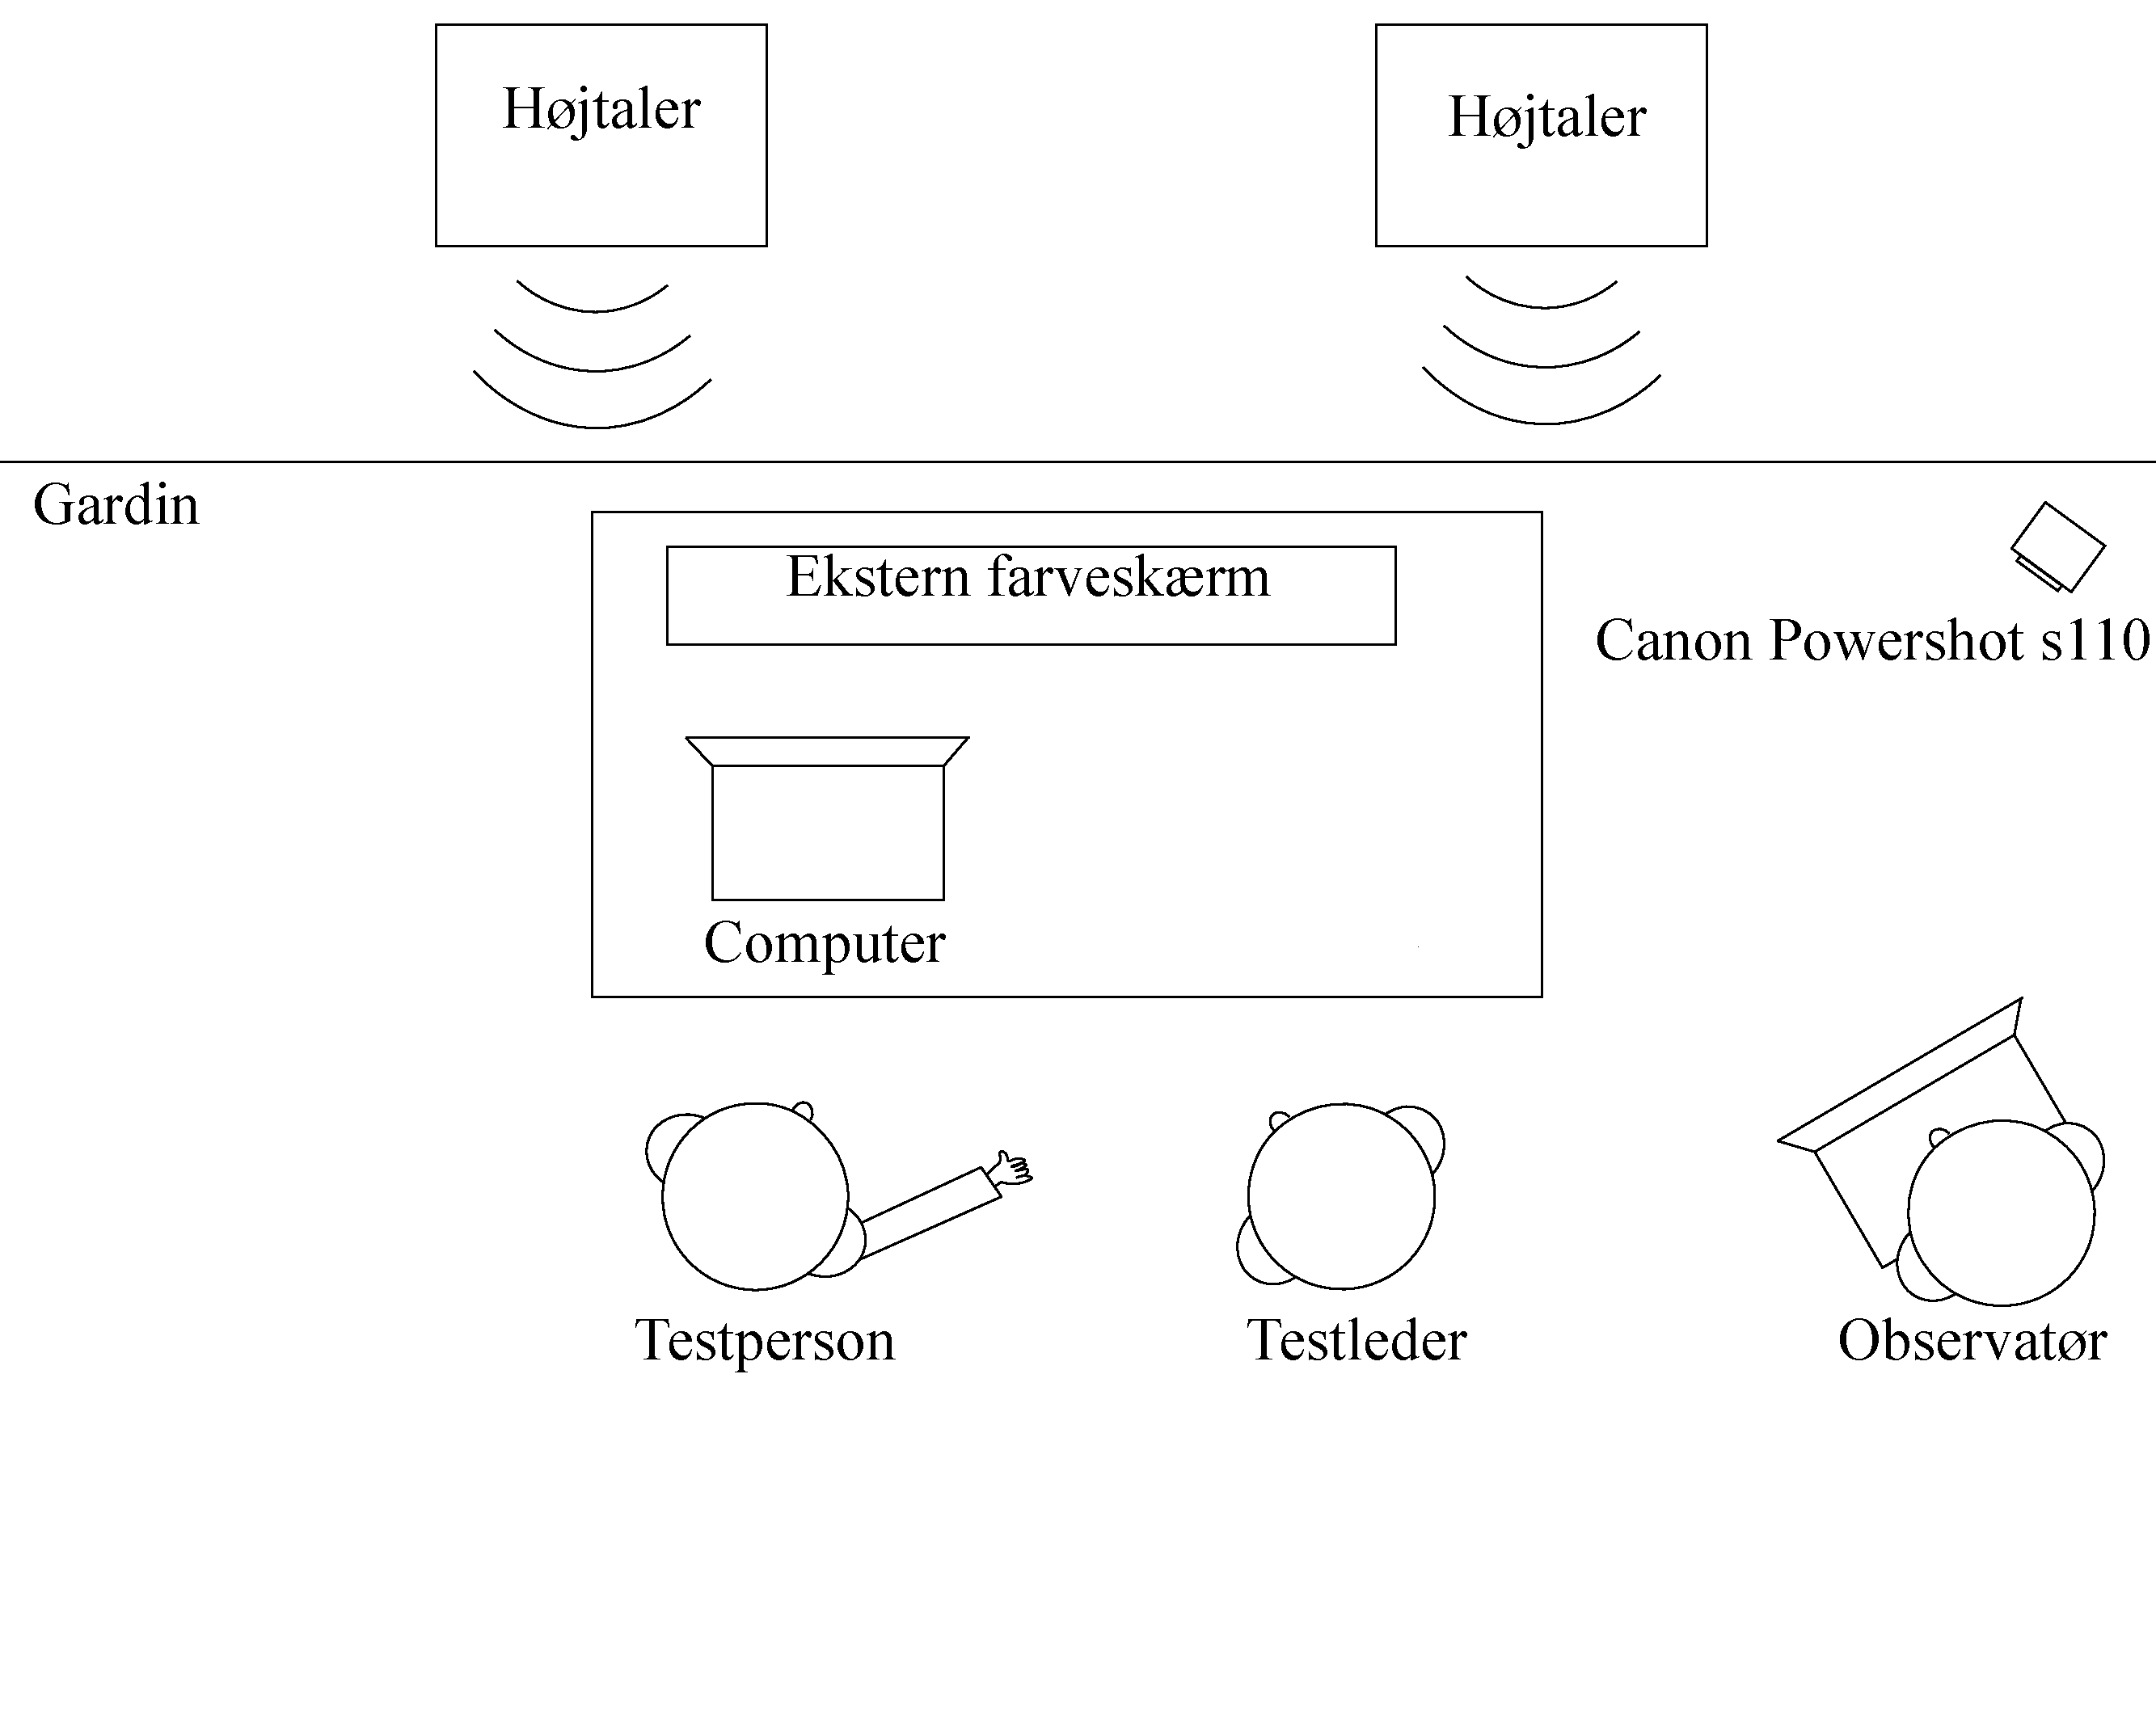
\includegraphics[resolution=300,width=0.8\textwidth]{Test1/TestopstillingPrePilot}
	\caption{Testopstilling hvor placeringen af udstyr, testleder, observatør og testperson fremgår.}
	\label{fig:TestopstillingPrePilot}
\end{figure}
\noindent
% 
Testen afvikles i Lytterummet B4-107 i akustikafdelingen på Aalborg Universitets, Fredrik Bajers Vej 7B. 
%